\documentclass[10pt,pdftex,aspectratio=1610]{beamer}
\usepackage{amsmath, amsthm, amssymb}
\usepackage{color}
\usepackage{hyperref}
\usepackage{subfigure}
\usepackage{tabularx}
\usepackage{ragged2e}
\usepackage{booktabs}
\usepackage{multirow}
\usepackage{natbib}
\usepackage{bbm}
\usepackage[listings, most]{tcolorbox}

\usecolortheme{dolphin}
\linespread{1.3}
\definecolor{nblue}{RGB}{0,0,128}

\bibliographystyle{ecta}
\setbeamercovered{transparent}

\newcolumntype{Y}{>{\RaggedRight\arraybackslash}X}
%\setbeamerfont{alerted text}{series=\bfseries}

\hypersetup{colorlinks=true, linkcolor=nblue,
citecolor=nblue, urlcolor=nblue, bookmarks=false,
pdfpagemode=UseNone,
pdfstartview={XYZ null null 1.0},
pdftitle={Heterogeneous Agent Trade},
pdfauthor={ Michael E. Waugh},
pdfkeywords={economics, trade, dynamics, quant econ, consumption, data science,
waugh, incomplete markets, inequality, Ricardo, julia, Armington, China, trade war, tariffs, python, matplotlib}}

%\usepackage[pdftex,colorlinks=true, bookmarks=false,
%pdfstartview={XYZ null null 1.0},
%pdftitle={Heterogeneous Agent Trade},
%pdfauthor={Michael E. Waugh},
%pdfkeywords={economics, trade, dynamics, quant econ, consumption, data science,
%waugh, incomplete markets, inequality, Ricardo, julia, Armington, China, trade war, tariffs, python, matplotlib},
%colorlinks=true,linkcolor=darkgray,citecolor=darkgray,urlcolor=darkgray,
%breaklinks]{hyperref}

\setbeamertemplate{navigation symbols}{}
\setbeamertemplate{footline}[frame number]
\setbeamertemplate{theorems}[numbered]
\setbeamertemplate{itemize subitem}[circle]
\setbeamertemplate{enumerate items}[default]

\setbeamerfont{frametitle}{size= \large}
\setbeamerfont{ framesubtitle }{size = \footnotesize}
\setbeamertemplate{frametitle}
{
\medskip
\smallskip
{\textsf{\underline{\insertframetitle\phantom{))))))))}}}}}
\setbeamertemplate{items}[circle]
\setbeamertemplate{itemize subitem}[circle]

\theoremstyle{definition}


\newtheorem{as}{Assumption}
\newtheorem{df}{Definition}
\newtheorem{lm}{Lemma}
\newtheorem{prp}{Proposition}

\tcolorboxenvironment{prp}{%
boxrule = 0mm, breakable, colframe=white,
before skip=5pt,after skip=5pt,
colback=gray!5!white,
top = 2mm,
bottom = 2mm%,
%borderline north={1pt}{1pt}{gray},
%borderline south={1pt}{1pt}{gray}
}

\tcolorboxenvironment{df}{%
boxrule = 0mm, breakable, colframe=white,
before skip=5pt,after skip=5pt,
colback=gray!5!white,
top = 2mm,
bottom = 2mm%,
%borderline north={1pt}{1pt}{gray},
%borderline south={1pt}{1pt}{gray}
}


\usepackage[normalem]{ulem}
\newcommand\redout{\bgroup\markoverwith
{\textcolor{red}{\rule[.5ex]{1pt}{1pt}}}\ULon}

\makeatletter
\def\blfootnote{\xdef\@thefnmark{}\@footnotetext}
\makeatother

%%%%%%%%%%%%%%%%%%%%%%%%%%%%%%%%%%%%%%%%%%%%%%%%%%%%%%%%%%%%%%%%%%%%%%%%%%%%%%%%%%%%%%%%%%%%%%%%%
%%%%%%%%%%%%%%%%%%%%%%%%%%%%%%%%%%%%%%%%%%%%%%%%%%%%%%%%%%%%%%%%%%%%%%%%%%%%%%%%%%%%%%%%%%%%%%%%%



\date{\today}

\begin{document}

\begin{frame}[t]
\frametitle{Price Gaps and Observables}
\footnotesize

\begin{table}[!t]
\footnotesize
\renewcommand{\arraystretch}{1.95}
\setlength {\tabcolsep}{2.5mm}
\begin{center}\label{tb:data_rslts}
\begin{tabular}[t]{l c c c }
\multicolumn{4}{c}{\normalsize \textbf{ Correlations of Price Gaps and Observables}}
\\
\hline
\hline
& \textbf{Distance} & \textbf{Border} & \textbf{Tariffs} \\
\cmidrule(r){2-2}  \cmidrule(lr){3-3} \cmidrule(lr){4-4}
Price gap, $d_{ni}$     & $\begin{array}{c}{\textbf{0.42}} \vspace{-.4cm}\\ \scriptstyle{[0.39,   \ 0.45]}\end{array}$ &
$\begin{array}{c}{\textbf{-0.18}} \vspace{-.4cm}\\ \scriptstyle{[-0.21,   \ -0.15]}\end{array}$
& $\begin{array}{c}{\textbf{0.34}} \vspace{-.4cm}\\ \scriptstyle{[0.31,   \ 0.36]}\end{array}$  \\
\hline
\end{tabular}
\\[0.75ex]
\parbox{4.5in}{\footnotesize This table pariwise correlation pooling all non-zero observations and the years 2004, 2011, 2017. Distancee and tariffs are in logarithims. 90-10 confidence intervals reported in brackets. }
\end{center}
\end{table}


\end{frame}


%%%%%%%%%%%%%%%%%%%%%%%%%%%%%%%%%%%%%%%%%%%%%%%%%%%%%%%%%%%%%%%%%%%%%%%%%%%%%%%%%%%%%%%%%%%%%%%%%
%%%%%%%%%%%%%%%%%%%%%%%%%%%%%%%%%%%%%%%%%%%%%%%%%%%%%%%%%%%%%%%%%%%%%%%%%%%%%%%%%%%%%%%%%%%%%%%%%

\begin{frame}[t]
\frametitle{Estimation Results}
\footnotesize

\begin{table}[!t]
\footnotesize
\renewcommand{\arraystretch}{1.85}
\setlength {\tabcolsep}{3.0mm}
\begin{center}\label{tb:data_rslts}
\begin{tabular}[t]{l c c c }
\multicolumn{4}{c}{\normalsize \textbf{ Estimation Results, Exactly Identified}}
\\
\hline
\hline
& \textbf{2004} & \textbf{2011} & \textbf{2017} \\
\cmidrule(r){2-2}  \cmidrule(lr){3-3} \cmidrule(lr){4-4}
Armington       & $\begin{array}{c}{\textbf{5.27}} \vspace{-.4cm}\\ \scriptstyle{[5.10,   \ 5.53]}\end{array}$ &
$\begin{array}{c}{\textbf{4.89}} \vspace{-.4cm}\\ \scriptstyle{[4.72,   \ 5.13]}\end{array}$ &
$\begin{array}{c}{\textbf{5.23}} \vspace{-.4cm}\\ \scriptstyle{[5.03,   \ 5.48]}\end{array}$ \\
EK              & $\begin{array}{c}{\textbf{4.19}} \vspace{-.4cm}\\ \scriptstyle{[4.04,   \ 4.33]}\end{array}$  &
$\begin{array}{c}{\textbf{3.93}} \vspace{-.4cm}\\ \scriptstyle{[3.80,   \ 4.07]}\end{array}$ &
$\begin{array}{c}{\textbf{4.25}} \vspace{-.4cm}\\ \scriptstyle{[4.11,   \ 4.39]}\end{array}$\\
BEJK            & $\begin{array}{c}{\textbf{3.34}} \vspace{-.4cm}\\ \scriptstyle{[3.21,   \ 3.47]}\end{array}$ &
$\begin{array}{c}{\textbf{3.17}} \vspace{-.4cm}\\ \scriptstyle{[3.05,   \ 3.29]}\end{array}$ &
  $\begin{array}{c}{\textbf{3.37}} \vspace{-.4cm}\\ \scriptstyle{[3.25,   \ 3.49]}\end{array}$ \\
\hline
\end{tabular}
\\[0.75ex]
\parbox{2.5in}{\footnotesize }
\end{center}
\end{table}


\end{frame}

%%%%%%%%%%%%%%%%%%%%%%%%%%%%%%%%%%%%%%%%%%%%%%%%%%%%%%%%%%%%%%%%%%%%%%%%%%%%%%%%%%%%%%%%%%%%%%%%%
%%%%%%%%%%%%%%%%%%%%%%%%%%%%%%%%%%%%%%%%%%%%%%%%%%%%%%%%%%%%%%%%%%%%%%%%%%%%%%%%%%%%%%%%%%%%%%%%%

\begin{frame}[t]
\frametitle{Estimation Results}
\footnotesize

\begin{table}[!t]
\footnotesize
\renewcommand{\arraystretch}{1.85}
\setlength {\tabcolsep}{1.75mm}
\begin{center}\label{tb:data_rslts}
\begin{tabular}[t]{l c c c c c c }
\multicolumn{7}{c}{\normalsize \textbf{ Estimation Results, Overidentified}}
\\
\hline
\hline
& \multicolumn{2}{c}{\textbf{2004}} & \multicolumn{2}{c}{\textbf{2011}} & \multicolumn{2}{c}{\textbf{2017}} \\
& Estimate of $\theta$ & J-Stat P-value & Estimate of $\theta$ & J-Stat P-value & Estimate of $\theta$ & J-Stat P-value \\
\cmidrule(r){2-3}  \cmidrule(lr){4-5} \cmidrule(lr){6-7}
Armington       & $\begin{array}{c}{\textbf{3.70}} \vspace{-.4cm}\\ \scriptstyle{[3.52,   \ 3.78]}\end{array}$ & $< 0.01$&
$\begin{array}{c}{\textbf{3.55}} \vspace{-.4cm}\\ \scriptstyle{[3.38,   \ 3.63]}\end{array}$ & $< 0.01$&
$\begin{array}{c}{\textbf{3.87}} \vspace{-.4cm}\\ \scriptstyle{[3.68,   \ 3.97]}\end{array}$ &$< 0.01$\\
EK              & $\begin{array}{c}{\textbf{4.07}} \vspace{-.4cm}\\ \scriptstyle{[3.97,   \ 4.15]}\end{array}$  & $0.61$&
$\begin{array}{c}{\textbf{4.26}} \vspace{-.4cm}\\ \scriptstyle{[4.16,   \ 4.35]}\end{array}$ & $< 0.01$&
$\begin{array}{c}{\textbf{4.38}} \vspace{-.4cm}\\ \scriptstyle{[4.28,   \ 4.47]}\end{array}$ & $< 0.01$\\
BEJK            & $\begin{array}{c}{\textbf{3.16}} \vspace{-.4cm}\\ \scriptstyle{[3.08,   \ 3.20]}\end{array}$ &$< 0.01$ &
$\begin{array}{c}{\textbf{3.21}} \vspace{-.4cm}\\ \scriptstyle{[3.12,   \ 3.26]}\end{array}$ &$< 0.01$ &
  $\begin{array}{c}{\textbf{3.33}} \vspace{-.4cm}\\ \scriptstyle{[3.24,   \ 3.38]}\end{array}$ & $< 0.01$\\
\hline
\end{tabular}
\\[0.75ex]
\parbox{2.5in}{\footnotesize }
\end{center}
\end{table}


\end{frame}

%%%%%%%%%%%%%%%%%%%%%%%%%%%%%%%%%%%%%%%%%%%%%%%%%%%%%%%%%%%%%%%%%%%%%%%%%%%%%%%%%%%%%%%%%%%%%%%%%
%%%%%%%%%%%%%%%%%%%%%%%%%%%%%%%%%%%%%%%%%%%%%%%%%%%%%%%%%%%%%%%%%%%%%%%%%%%%%%%%%%%%%%%%%%%%%%%%%

\begin{frame}[t]
\frametitle{Estimation Results}
\footnotesize

\begin{table}[!t]
\footnotesize
\renewcommand{\arraystretch}{1.85}
\setlength {\tabcolsep}{3.0mm}
\begin{center}\label{tb:data_rslts}
\begin{tabular}[t]{l c c c }
\multicolumn{4}{c}{\normalsize \textbf{ Estimation Results, Endogenous Variety Models}}
\\
\hline
\hline
& \textbf{2004} & \textbf{2011} & \textbf{2017} \\
\cmidrule(r){2-2}  \cmidrule(lr){3-3} \cmidrule(lr){4-4}
Krugman       & $\begin{array}{c}{\textbf{5.27}} \vspace{-.4cm}\\ \scriptstyle{[5.10,   \ 5.53]}\end{array}$ &
$\begin{array}{c}{\textbf{4.89}} \vspace{-.4cm}\\ \scriptstyle{[4.72,   \ 5.13]}\end{array}$ &
$\begin{array}{c}{\textbf{5.23}} \vspace{-.4cm}\\ \scriptstyle{[5.03,   \ 5.48]}\end{array}$ \\
Melitz             & $\begin{array}{c}{\textbf{3.65}} \vspace{-.4cm}\\ \scriptstyle{[3.19,   \ 3.99]}\end{array}$  &
$\begin{array}{c}{\textbf{3.19}} \vspace{-.4cm}\\ \scriptstyle{[2.73,   \ 3.44]}\end{array}$ &
$\begin{array}{c}{\textbf{3.23}} \vspace{-.4cm}\\ \scriptstyle{[2.82,   \ 3.54]}\end{array}$\\
\hline
\end{tabular}
\\[0.75ex]
\parbox{2.5in}{\footnotesize }
\end{center}
\end{table}


\end{frame}


%%%%%%%%%%%%%%%%%%%%%%%%%%%%%%%%%%%%%%%%%%%%%%%%%%%%%%%%%%%%%%%%%%%%%%%%%%%%%%%%%%%%%%%%%%%%%%%%%
%%%%%%%%%%%%%%%%%%%%%%%%%%%%%%%%%%%%%%%%%%%%%%%%%%%%%%%%%%%%%%%%%%%%%%%%%%%%%%%%%%%%%%%%%%%%%%%%%

\begin{frame}[t]
\frametitle{Estimation Results}
\footnotesize

\begin{table}[!t]
\footnotesize
\renewcommand{\arraystretch}{1.85}
\setlength {\tabcolsep}{1.75mm}
\begin{center}\label{tb:data_rslts}
\begin{tabular}[t]{l c c c c c c }
\multicolumn{7}{c}{\normalsize \textbf{ Estimation Results, Overidentified, Endogenous Variety Models}}
\\
\hline
\hline
& \multicolumn{2}{c}{\textbf{2004}} & \multicolumn{2}{c}{\textbf{2011}} & \multicolumn{2}{c}{\textbf{2017}} \\
& Estimate of $\theta$ & J-Stat P-value & Estimate of $\theta$ & J-Stat P-value & Estimate of $\theta$ & J-Stat P-value \\
\cmidrule(r){2-3}  \cmidrule(lr){4-5} \cmidrule(lr){6-7}
Krugman       & $\begin{array}{c}{\textbf{3.70}} \vspace{-.4cm}\\ \scriptstyle{[3.52,   \ 3.78]}\end{array}$ & $< 0.01$&
$\begin{array}{c}{\textbf{3.55}} \vspace{-.4cm}\\ \scriptstyle{[3.38,   \ 3.63]}\end{array}$ & $< 0.01$&
$\begin{array}{c}{\textbf{3.87}} \vspace{-.4cm}\\ \scriptstyle{[3.68,   \ 3.97]}\end{array}$ &$< 0.01$\\
Melitz            & $\begin{array}{c}{\textbf{3.73}} \vspace{-.4cm}\\ \scriptstyle{[3.48,   \ 3.92]}\end{array}$  & $0.85$&
$\begin{array}{c}{\textbf{3.12}} \vspace{-.4cm}\\ \scriptstyle{[2.80,   \ 3.45]}\end{array}$ & $0.13$&
$\begin{array}{c}{\textbf{3.03}} \vspace{-.4cm}\\ \scriptstyle{[2.60,   \ 3.85]}\end{array}$ & $0.85$\\
\hline
\end{tabular}
\\[0.75ex]
\parbox{2.5in}{\footnotesize }
\end{center}
\end{table}


\end{frame}


%%%%%%%%%%%%%%%%%%%%%%%%%%%%%%%%%%%%%%%%%%%%%%%%%%%%%%%%%%%%%%%%%%%%%%%%%%%%%%%%%%%%%%%%%%%%%%%%
%%%%%%%%%%%%%%%%%%%%%%%%%%%%%%%%%%%%%%%%%%%%%%%%%%%%%%%%%%%%%%%%%%%%%%%%%%%%%%%%%%%%%%%%%%%%%%%%
\begin{frame}[t]
\frametitle{Estimation Results}
\begin{figure}[!t]
\centering{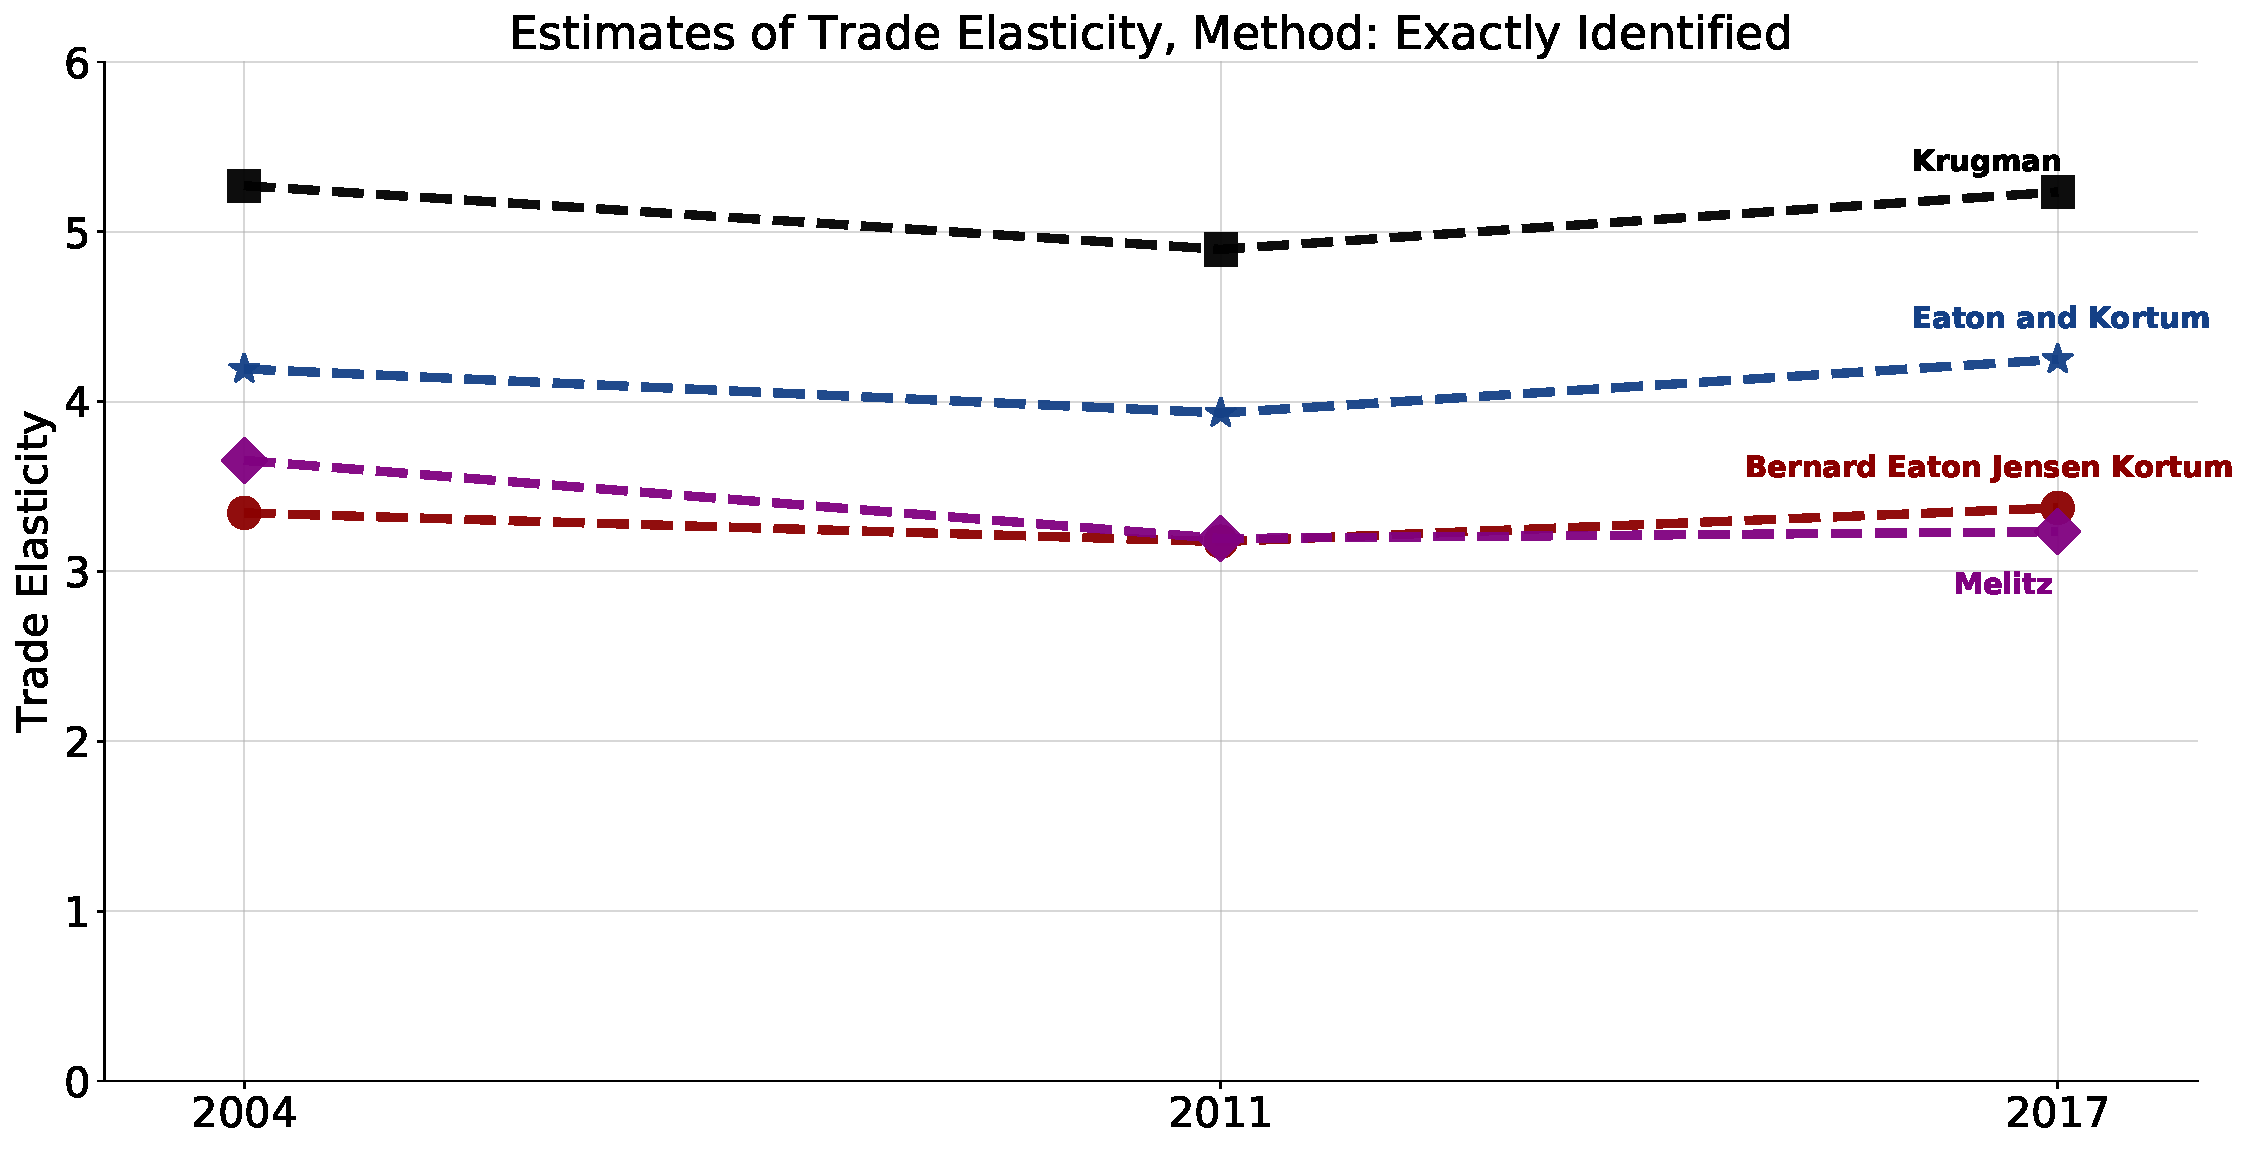
\includegraphics[scale = .39]{../results/model-year-exact.pdf}}
\end{figure}
\end{frame}

%%%%%%%%%%%%%%%%%%%%%%%%%%%%%%%%%%%%%%%%%%%%%%%%%%%%%%%%%%%%%%%%%%%%%%%%%%%%%%%%%%%%%%%%%%%%%%%%
%%%%%%%%%%%%%%%%%%%%%%%%%%%%%%%%%%%%%%%%%%%%%%%%%%%%%%%%%%%%%%%%%%%%%%%%%%%%%%%%%%%%%%%%%%%%%%%%
\begin{frame}[t]
\frametitle{Estimation Results}
\begin{figure}[!t]
\centering{
\includegraphics[scale = .39]{../results/model-year-over.pdf}}
\end{figure}
\end{frame}


%%%%%%%%%%%%%%%%%%%%%%%%%%%%%%%%%%%%%%%%%%%%%%%%%%%%%%%%%%%%%%%%%%%%%%%%%%%%%%%%%%%%%%%%%%%%%%%%%
%%%%%%%%%%%%%%%%%%%%%%%%%%%%%%%%%%%%%%%%%%%%%%%%%%%%%%%%%%%%%%%%%%%%%%%%%%%%%%%%%%%%%%%%%%%%%%

\end{document}













